%----------------------------------------------------------------------------------------
%	PACKAGES AND OTHER DOCUMENT CONFIGURATIONS
%----------------------------------------------------------------------------------------

\documentclass[
10pt, % Main document font size
a4paper, % Paper type, use 'letterpaper' for US Letter paper
oneside, % One page layout (no page indentation)
%twoside, % Two page layout (page indentation for binding and different headers)
headinclude,footinclude, % Extra spacing for the header and footer
BCOR5mm, % Binding correction
]{scrartcl}

%----------------------------------------------------------------------------------------
%	REQUIRED PACKAGES
%----------------------------------------------------------------------------------------

\usepackage[german]{babel}

\usepackage[
nochapters, % Turn off chapters since this is an article        
beramono, % Use the Bera Mono font for monospaced text (\texttt)
eulermath,% Use the Euler font for mathematics
pdfspacing, % Makes use of pdftex’ letter spacing capabilities via the microtype package
dottedtoc % Dotted lines leading to the page numbers in the table of contents
]{classicthesis} % The layout is based on the Classic Thesis style

\usepackage{arsclassica} % Modifies the Classic Thesis package

\usepackage[T1]{fontenc} % Use 8-bit encoding that has 256 glyphs

\usepackage[utf8]{inputenc} % Required for including letters with accents

\usepackage{graphicx} % Required for including images
\graphicspath{{Figures/}} % Set the default folder for images

\usepackage{enumitem} % Required for manipulating the whitespace between and within lists

\usepackage{lipsum} % Used for inserting dummy 'Lorem ipsum' text into the template

\usepackage{subfig} % Required for creating figures with multiple parts (subfigures)

\usepackage{amsmath,amssymb,amsthm} % For including math equations, theorems, symbols, etc

\usepackage{varioref} % More descriptive referencing

\usepackage{listings}

%----------------------------------------------------------------------------------------
%	THEOREM STYLES
%---------------------------------------------------------------------------------------

\theoremstyle{definition} % Define theorem styles here based on the definition style (used for definitions and examples)
\newtheorem{definition}{Definition}

\theoremstyle{plain} % Define theorem styles here based on the plain style (used for theorems, lemmas, propositions)
\newtheorem{theorem}{Theorem}

\theoremstyle{remark} % Define theorem styles here based on the remark style (used for remarks and notes)

%----------------------------------------------------------------------------------------
%	HYPERLINKS
%---------------------------------------------------------------------------------------

\hypersetup{
%draft, % Uncomment to remove all links (useful for printing in black and white)
colorlinks=true, breaklinks=true, bookmarks=true,bookmarksnumbered,
urlcolor=webbrown, linkcolor=RoyalBlue, citecolor=webgreen, % Link colors
pdftitle={}, % PDF title
pdfauthor={\textcopyright}, % PDF Author
pdfsubject={}, % PDF Subject
pdfkeywords={}, % PDF Keywords
pdfcreator={pdfLaTeX}, % PDF Creator
pdfproducer={LaTeX with hyperref and ClassicThesis} % PDF producer
}

%\hyphenation{Fortran hy-phen-ation} % Specify custom hyphenation points in words with dashes where you would like hyphenation to occur, or alternatively, don't put any dashes in a word to stop hyphenation altogether

%----------------------------------------------------------------------------------------
%	TITLE AND AUTHOR(S)
%----------------------------------------------------------------------------------------

\title{\normalfont\spacedallcaps{Festmanager 2013}} % The article title

\author{\spacedlowsmallcaps{Freiwillige Feuerwehr Karlstetten\textsuperscript{1}}} % The article author(s) - author affiliations need to be specified in the AUTHOR AFFILIATIONS block

\date{} % An optional date to appear under the author(s)

%----------------------------------------------------------------------------------------

\begin{document}

%----------------------------------------------------------------------------------------
%	HEADERS
%----------------------------------------------------------------------------------------

\renewcommand{\sectionmark}[1]{\markright{\spacedlowsmallcaps{#1}}} % The header for all pages (oneside) or for even pages (twoside)
%\renewcommand{\subsectionmark}[1]{\markright{\thesubsection~#1}} % Uncomment when using the twoside option - this modifies the header on odd pages
\lehead{\mbox{\llap{\small\thepage\kern1em\color{halfgray} \vline}\color{halfgray}\hspace{0.5em}\rightmark\hfil}} % The header style

\pagestyle{scrheadings} % Enable the headers specified in this block

%----------------------------------------------------------------------------------------
%	TABLE OF CONTENTS & LISTS OF FIGURES AND TABLES
%----------------------------------------------------------------------------------------

\maketitle % Print the title/author/date block

\setcounter{tocdepth}{2} % Set the depth of the table of contents to show sections and subsections only

\tableofcontents % Print the table of contents

%\listoffigures % Print the list of figures

%\listoftables % Print the list of tables

%----------------------------------------------------------------------------------------
%	ABSTRACT
%----------------------------------------------------------------------------------------

%\section*{Abstract} % This section will not appear in the table of contents due to the star (\section*)
%\lipsum[1] % Dummy text

%----------------------------------------------------------------------------------------
%	AUTHOR AFFILIATIONS
%----------------------------------------------------------------------------------------

{\let\thefootnote\relax\footnotetext{\textsuperscript{1} \textit{Entwickler: FT Dominik Macher, OBI Markus Dürauer}}}



%----------------------------------------------------------------------------------------
%	INTRODUCTION
%----------------------------------------------------------------------------------------

%\newpage % Start the article content on the second page, remove this if you have a longer abstract that goes onto the second page
\section{Übersicht}
\textsl{FestManager 2013} ist eine von der Freiwilligen Feuerwehr Karlstetten entwickelte Applikation und entspricht dem Softwareteil für ein Boniersystem mit Bondruckern. 

\subsection{Software}
Die Software besteht im Grunde aus zwei Client-Applikationen und einer Access-Datenbank. Die Client-Applikationen wurden in \textsl{C\#.NET} für Microsoft Windows Clients entwickelt. \\
Die Datenbank dient zum Abspeichern aller Bestellungen. Die beiden Client-Applikationen bieten die folgenden Funktionen:
\begin{description}
	\item[FestManager Bestellung:] Diese Applikation dient der Aufnahme von Bestellungen (z.B. Kellner kommt zur Kassa und "`bestellt"). \\ Dabei werden seine aufgenommenen Artikel vom Kassa-Personal in die Applikation eingegeben. Nach Abschluss der Bestellung werden die Bons auf den jeweiligen Bondruckern ausgedruckt.
	\item[FestManager Abrechnung:] Diese Applikation dient der Abrechnung von Kellner-Personal. Speziell um die Mittagszeit ist es den einzelnen Kellnern aufgrund von Zeitdruck nicht möglich alle Bestellungen direkt an der Kassa zu zahlen. Daher wird zu einem späteren Zeitpunkt abgerechnet. \\ Das System merkt sich dabei alle, seit der letzten Kellnerabrechnung getätigten Bestellungen.
\end{description}

\subsection{Technische Daten, Anforderungen}
\begin{itemize}
	\item Microsoft Windows 2000, ME, XP, 7, 8
	\item Microsoft .NET Framework 2.0
	\item \textit{Optional: Microsoft Access zum Manuellen Editieren der Datenbank}
\end{itemize}

\subsection{Funktionen}
Einige der möglichen Funktionen sind aufgelistet:
\begin{itemize}
	\item Rasche Eingabe von Bestellungen mittels programmierbarer Tastatur
	\item Getrennte Ausgabestellen: Jeder Artikel wird einer Ausgabestelle zugeordnet (z.B. Schank, Küche, Weinbar, ...). Bei Abschließen einer Bestellung werden am jeweiligen Bondrucker der Ausgabestelle nur die zugeordneten Artikel ausgedruckt.
	\item Rechnung drucken: Jede Bestellung kann per Knopfdruck nach Abschließen erneut ausgedruckt werden, falls Kunden eine Rechnung wünschen. Diese Rechnung enthält alle Artikel der Bestellung, unabhängig von der Ausgabestelle.
	\item Direktverkauf (Beleg doppelt drucken): Diese Funktion ermöglicht es, dass bei Direktverkauf automatisch eine separate Rechnung ausgedruckt wird.
	\item Storno: Artikel können während der Eingabe von Bestellungen storniert werden. Weiters können Artikel nach Abschluss einer Bestellung auch in einer separaten Bestellung mittels Storno-Symbol storniert werden. Die Abrechnungs-Applikation ermöglicht auch die Stornierung von ganzen Bestellungen.
	\item Einpacken: Möchte ein Kunde seine Speisen eingepackt, so erscheint am Bondrucker bei der Ausgabestelle ein eigenes Symbol. Somit findet der Kunde seine Speisen bei Abholung bereits eingepackt vor.
\end{itemize}


\subsection{Hardware}
Neben der Software gehören auch noch Geräte zum Boniersystem:
\begin{itemize}
	\item Bondrucker (Anschluss Parallel bzw. Netzwerk über Printserver)
	\item programmierbare Tastatur, für die rasche Eingabe bei der Bestell-Applikation
\end{itemize}

\subsection{Architektur: Zusammenspiel Software und Hardware}
Das System ist prinzipiell Multi-User-fähig aufgebaut, d.h. dass Applikationen von verschiedenen Clients gleichzeitig auf eine gemeinsame Datenbank zugreifen können. \\
Im Prinzip können beliebig viele Bondrucker verwendet werden, welche über Netzwerk verbunden sind. Hat man kein Netzwerk zur Verfügung, so kann man die Drucker (max. 2) auf direkt an einen PC anschließen. Der große Vorteil in der Netzwerkverkabelung liegt in der Verkabelung von großen Strecken, d.h. dass die Bondrucker an verschiedenen Orten im Festgelände positioniert werden können und über LAN miteinander kommunizieren. \\
Bei Verwendung von mehreren PCs eignet sich die Benutzung eines zentralen Servers (File-Share), auf dem die Datenbank liegt. Es empfiehlt sich ebenfalls periodisch Sicherungen von der Datenbank durchzuführen. Hat man keinen zentralen Rechner zum Freigeben der Datenbank (z.B. im Feld), so kann die Datenbank auch direkt auf einem PC gespeichert und dem anderen PC freigegeben werden. \\

Zwei Beispiele für mögliche Anordnung der Netzwerkkomponenten sind in den folgenden Abbildungen ersichtlich:

\begin{figure}[h]
\centering 
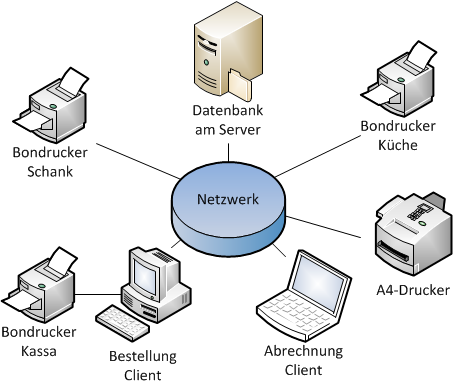
\includegraphics[width=0.5\columnwidth]{figures/mit_server.png} 
\caption{Architektur mit Server} 
\label{fig:mit_server} 
\end{figure}

\begin{figure}[h]
\centering 
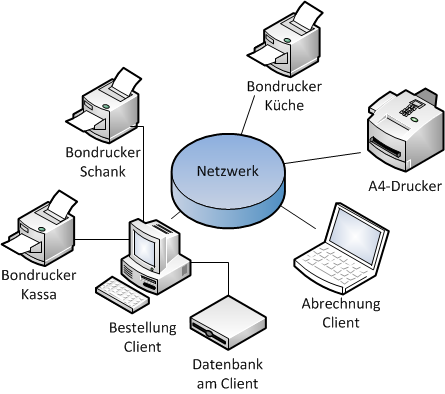
\includegraphics[width=0.5\columnwidth]{figures/ohne_server.png} 
\caption{Architektur ohne Server} 
\label{fig:ohne_server} 
\end{figure}



%----------------------------------------------------------------------------------------
%	configuration
%----------------------------------------------------------------------------------------
\newpage
\section{Konfiguration}

\subsection{CONFIG Datei}
Jede Client-Applikation (Bestellung oder Abrechnung) besteht aus einer ausführbaren \texttt{.exe} Datei und einer \texttt{.exe.config} Datei zum konfigurieren der Applikation. Der Inhalt einer solchen config-Datei ist im folgenden Abschnitt dargestellt.

\lstset{
  language=XML,
	basicstyle=\footnotesize,
  morekeywords={encoding,
    xs:schema,xs:element,xs:complexType,xs:sequence,xs:attribute}
}
\begin{lstlisting}
<?xml version="1.0" encoding="utf-8" ?>
<configuration>
    <configSections>
        ...
    </configSections>
    <connectionStrings>
        <add name="FestManager_Bestellung.Properties.Settings.connectionString"
            connectionString="Provider=Microsoft.Jet.OLEDB.4.0;Data Source=D:\fest2015.mdb" />
    </connectionStrings>
    <userSettings>
        <FestManager_Bestellung.Properties.Settings>
            <setting name="organisation" serializeAs="String">
                <value>FF-Karlstetten</value>
            </setting>
            <setting name="printDirektverkaufTwice" serializeAs="String">
                <value>False</value>
            </setting>
        </FestManager_Bestellung.Properties.Settings>
    </userSettings>
</configuration>
\end{lstlisting}

\subsection{Konfiguration der Datenbank}
Die Access-Datenbank-Datei hat die Endung \texttt{.mdb}. Vor Verwendung der Client-Applikationen muss der Pfad zur Datenbank-Datei angepasst werden. Dazu muss die Zeile in der config-Datei mit \texttt{Data Source=FILEPATH.mdb} richtig gesetzt werden.

\subsection{Konfigurationsparameter}
Die meisten beschriebenen Funktionen können ebenfalls in der config-Datei aktiviert oder deaktiviert werden und bestimmen somit das Verhalten der jeweiligen Client-Applikation. Jede Konfiguration wird dabei durch ein \texttt{<setting>} repräsentiert. Ein Beispiel ist die Konfiguration der \texttt{organisation} mit Wert "`FF-Karlstetten"'. 


\begin{table}[h]
\footnotesize
\begin{tabular}{|l|l|l|}
\hline
Funktion (setting-name) & Standard-Wert (value) & Beschreibung \\
\hline
\hline
organisation & FF-Karlstetten & Name der Organisation \\
\hline
printDirektverkaufTwice & False & Automatische Rechnung für Direktverkauf \\
\hline
direktverkaufPersonalId & 1 & vordefinierte Personal-Nr. für Direktverkauf \\
\hline
direktverkaufAusgabestelleId & 0 & Ausgabestelle für Direktverkauf-Rechnungen \\
\hline
printStornoOrders & True & Storno-Bestellungen drucken / nicht drucken \\
\hline
stornoSymbol & † & Storno-Symbol für Bons \\
\hline
groupElementsBeforePrint & True & Gleiche Artikel beim Bondruck zusammenfassen \\
\hline
einpackenSymbol & $\triangle$ & Einpacken-Symbol für Bons \\
\hline
tableNumbers & True & Tischnummern-Eingabe aktiv / nicht aktiv \\
\hline
\end{tabular}
\end{table}


%----------------------------------------------------------------------------------------
%	CONTACT
%----------------------------------------------------------------------------------------

\newpage
\section{Kontakt}
\subsection{Copyright}
Freiwillige Feuerwehr Karlstetten\\
3121 Karlstetten\\
Wachaustraße 5

\subsection{Erreichbarkeit}
Email: office@feuerwehr-karlstetten.org




%----------------------------------------------------------------------------------------

\end{document}